%
% ─── CAPITULO 3: CONJUNTOS DE JULIA Y MANDELBROT ────────────────────────────────
%

Terminamos el capítulo \ref{chap:iteracion} fijándonos en la autosimilaridad de las imágenes que nos proporcionaba la aplicación del método de Newton en ciertas funciones complejas para deducir las cuencas de atracción de las distintas funciones. Pudimos comprobar que a pesar de ser imágenes que no son totalmente autosimilares, por lo que no son fractales en el sentido estricto, contienen fragmentos que sí lo son. Este mismo hecho se produce en los conjuntos de Julia y en el conjunto de Mandelbrot. Podemos observar este hecho en las imágenes \ref{fig:julia-intro}, que son nuestros primeros dos ejemplos de conjuntos de Julia.

\begin{figure}[ht]
    \centering
    \begin{tabular}{cc}
      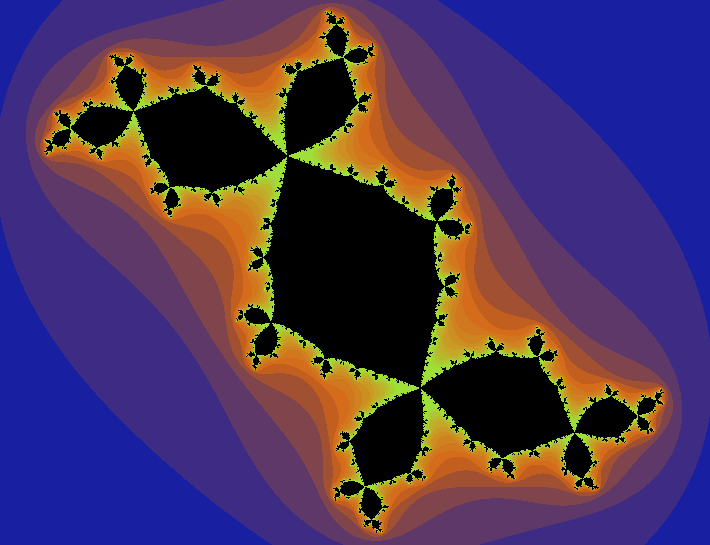
\includegraphics[scale=0.28]{./img/C3/julia-intro-2.png} &   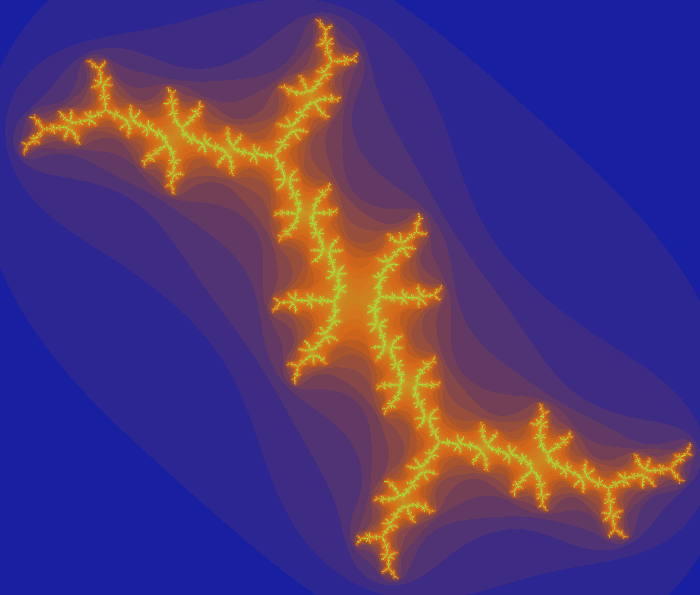
\includegraphics[scale=0.255]{./img/C3/julia-intro-1.png} \\
    (a) Conjunto de Julia conexo & (b) Conjunto de Julia no conexo  \\[6pt]
    \end{tabular}
    \caption{Primeras imágenes de conjuntos de Julia}
    \label{fig:julia-intro}
\end{figure}

Una notable diferencia entre las imágenes \ref{fig:julia-intro} se encuentra en que mientras en la imagen (a) se puede percibir cierta conexión en el conjunto, esta desaparece en el caso de la imagen (b). Precisamente en esa distinción reside la génesis del conocido \textit{conjunto de Mandelbrot}, que podemos también ver por primera vez, junto con algunas de sus autosimilaridades, en las imágenes \ref{fig:mandelbrot-intro}.

\begin{figure}[ht]
  \centering
  \begin{tabular}{cc}
    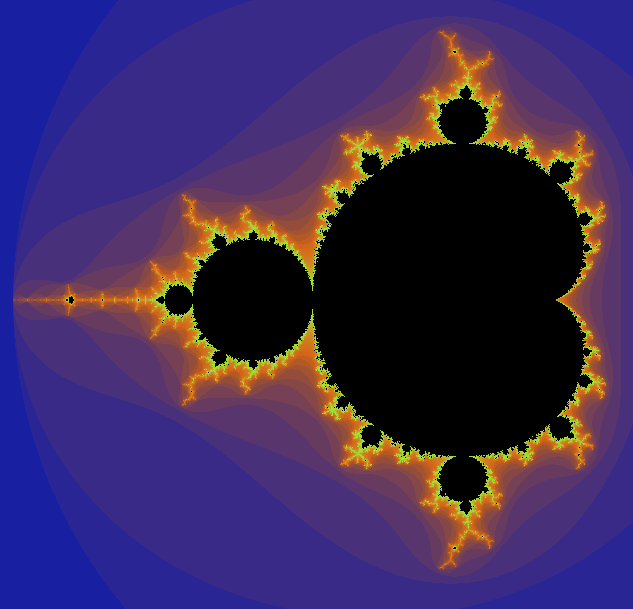
\includegraphics[scale=0.28]{./img/C3/mandelbrot-intro.png} &   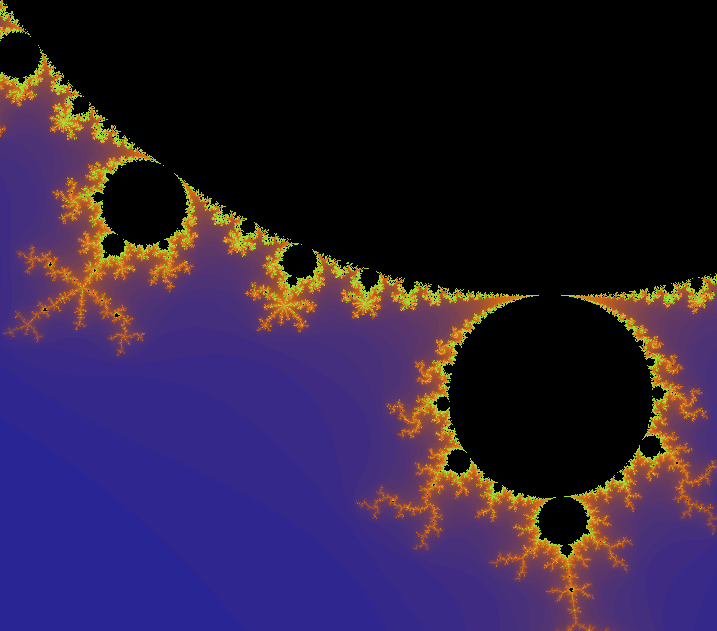
\includegraphics[scale=0.255]{./img/C3/detalle-Mandelbrot.png} \\
  (a) Conjunto completo & (b) Detalle ampliado  \\[6pt]
  \end{tabular}
    \caption{Primeras imágenes del conjunto de Mandelbrot}
    \label{fig:mandelbrot-intro}
\end{figure}

En este capítulo aprenderemos qué elementos componen estos conjuntos, y cómo llegar a estas imágenes tan llamativas.

\section{Iteración convergente y no convergente}

Recordamos que en el capítulo \refname{chap:iteracion}, a partir de una función analítica $f:\C\longrightarrow\C$, se le aplicaba una transformación $N_f(z)$ de forma que en muchos casos la iteración de dicha función era convergente independientemente del término $z_0\in\C$ inicial. Sin embargo recordemos que la iteración de una función cualquiera $f$ no siempre es convergente, como pudimos comprobar en el ejemplo situado al comienzo de la sección \ref{subsection:convergencia-punto-fijo}, en el que comprobamos que las iteradas de la función $f(z)=z^2$ divergen siempre que $|z_0|>1$, convergen a $0$ si $|z_0|<1$ y quedan encerradas en $S^1$ en caso de que $|z_0|=1$. Otro posible comportamiento es el cíclico, como el que tienen las iteradas de la función $g(z)=z\cdot i$ en $z_0=1$, que si nos fijamos, $O_g(1)=\{1,i,-1,-i,1,\dots\}$. 

Un último caso de posible comportamiento de una órbita son las órbitas caóticas, en las cuales no se percibe ningún patrón y además es muy sensible a las condiciones iniciales, fijémonos en lo que ocurre en el caso de la función $h(z)=z^2-1.9$ si miramos sus órbitas en $z_0=0,0.1$:

\begin{verbatim}
In[]:= h[z_] := z^2 - 1.9;
    NestList[h, 0.1, 20]
    NestList[h, 0.0, 20]


Out[]= {0.1, -1.89, 1.6721, 0.895918, -1.09733, -0.695866,
    -1.41577, 0.104404, -1.8891, 1.6687, 0.884552, -1.11757, 
    -0.651043, -1.47614, 0.279, -1.82216, 1.42026, 0.117148, 
    -1.88628, 1.65804, 0.849092}

Out[]= {0., -1.9, 1.71, 1.0241, -0.851219, -1.17543, -0.518374, 
  -1.63129, 0.761102, -1.32072, -0.155688, -1.87576, 1.61848, 
  0.719477, -1.38235, 0.0109007, -1.89988, 1.70955, 1.02256, 
  -0.854379, -1.17004}
\end{verbatim}

No se observa ningún patrón de convergencia y además, a pesar de ser semillas muy cercanas, las órbitas son muy diferentes.

La dicotomía existente entre qué $z_0$ iniciales hacen que las iteradas de una función coverga o no, restringida a cierta familia de funciones es la que define a los distintos conjuntos de Julia. Presentamos por tanto, para cada $c\in\C$, la familia de funciones
\begin{equation}
  P_c(z) = z^2 +c \ \ \forall z\in\C
\end{equation}

Nuestro objetivo es entonces clasificar para qué $z_0\in\C$, las iteradas $\{P_c^n(z_0)\}$ convergen, divergen, ciclan, o tienen posiblemente un comportamiento caótico.

\section{Conjuntos de Julia}

Sin dejar de tener en cuenta la familia de funciones $\{P_c(z)\}_{c\in\C}$ introducimos la siguiente definición.

\begin{definicion}
  Dado un número complejo $c\in\C$ fijo consideramos $P_c(z)=z^2+c$. Entonces:
  \begin{itemize}
    \item Se denomina \textbf{conjunto de puntos de escape}, y denotamos como $\mathsf{E}_c$ al conjunto de puntos cuyas iteradas divergen, es decir:
    $$
    \mathsf{E}_c = \{z_0\in\C: \{|P_c^n(z_0)|\}\rightarrow \infty \}
    $$
    \item  Se denomina \textbf{conjunto de puntos prisioneros}, y denotamos como $\mathsf{P}_c$ al conjunto de puntos cuyas iteradas no divergen, por lo que es el complemento de $\mathsf{E}_c$.
  \end{itemize}
\end{definicion}

A partir de estas dos definiciones, que insisten en clasificar los puntos del plano complejo entre de escape o prisioneros según su órbita, podemos introducir la definición que esperábamos.

\textit{He buscado información acerca de la duda que le planteé y ya tendría material para completar formalmente este apartado. Sin embargo, creo que es un poco técnica y realmente no termino de entenderla bien. La realidad es que se define el conjunto de Julia como el conjunto de puntos en los que la dinámica es caótica y por una serie de resultados acaba siendo equivalente a estas definiciones más sencillas. Pero para llegar a eso hay que meter artillería un poco pesada y quizá un poco fuera de contexto. Podemos verlo juntos y en función decidir.}

\begin{definicion}[Conjunto de Julia]
Dado un número $c\in\C$, se define su \textbf{conjunto de Julia}, y se denota como $\mathsf{J}_c$ a la frontera de $\mathsf{E}_c$. Es en este conjunto donde las iteradas tienen un comportamiento caótico. Se denomina \textbf{conjunto de Fatou} al complemento del conjunto de Julia.
\end{definicion}



\begin{ejemplo}
  En el caso $c=0$, es decir, $P_0(z)=z^2$, sabemos ya que $E_c=S^1$, pues precisamente es $S^1$ la frontera entre los puntos cuyas iteradas divergen o convergen a $0$.
\end{ejemplo}

\begin{observacion}
  Fijémonos por tanto que hay tantos conjuntos de Julia como números complejos, al poder asociar a cada número complejo un conjunto de puntos prisioneros, de escape, y por tanto un conjunto de Julia.
\end{observacion}

\subsection{Representación gráfica de los conjuntos de Julia}

Tenemos entonces una definición de los conjuntos de Julia, pero aparentemente está muy alejada de las imágenes \ref{fig:julia-intro} que presentamos en la introducción. La forma de llegar a ellas es similar a la que utilizamos para graficar las imágenes que utilizaban la velocidad de convergencia en el capítulo \ref{chap:iteracion}. Sin embargo, y al contrario que al utilizar el método de Newton, ahora no tenemos ningún tipo de convergencia asegurada, por lo que el método de aplicar iteradas hasta encontrar un patrón no es el más correcto. Debemos por tanto encontrar una manera eficiente de clasificar cada punto del plano como prisionero o de escape. 

Para ello podemos fijarnos en que la operación de elevar $z_n$ al cuadrado prima sobre la de sumar una constante $c$ siempre que el módulo $|z_n|$ sea 'suficientemente grande'. Procedemos entonces a enunciar el siguiente resultado:

\begin{teorema}
  Dado un $c\in\C$, consideramos la función $P_c(z)=z^2+c$. Si un número $z_0\in\C$ verifica que $|z_0|>\max\{|c|,2\}$, entonces $z_0$ es un punto de escape. Al número $e_c=\max\{|c|,2\}$ se le denomina \textit{número de escape}.
\end{teorema}
\begin{proof}
  Supongamos que $|z_0|>e_c=\max\{|c|,2\}$, por tanto necesariamente debe existir un número $\varepsilon>0$ tal que $|z_0| = 2 + \varepsilon$. Aplicamos entonces la cadena de desigualdades siguiente:
  \begin{eqnarray*}
    |P_c(z_0)| = |z_0^2 + c| & \geq & |z_0^2| - |c|\text{  (Propiedades del módulo)} \\
    & = & |z_0|^2 - c \\
    & \geq & |z_0|^2 - |z_0|\text{  (Porque } |z_0|>|c| \text{)} \\
    & = & (|z_0|-1)|z_0| \\
    & = & (1 + \varepsilon)|z_0|
  \end{eqnarray*}

  Por tanto tenemos que $|P_c(z_0)|\geq(1 + \varepsilon)|z_0|$, por lo que en cada iteración el módulo aumenta $1+\varepsilon$ unidades, que es mayor que uno, es decir, $|P_c^k(z_0)|\geq(1+\varepsilon)^k|z_0|$, por lo que la sucesión diverge y $z_0$ es un punto de escape. 
\end{proof}

Podemos aplicar este teorema para programar un algoritmo que grafique conjuntos de Julia. Para ello, fijamos un número $M\in\N$ que será el máximo de iteraciones que se aplicarán en cada punto antes de decidir si el punto es prisionero o de escape. Si pasadas esas $M$ iteraciones el módulo de $z_0$ no ha alcanzado el número de escape $e_c$ entonces consideramos que $z_0$ es un punto prisionero. En caso contrario, en el momento que se alcance el número de escape cesarán las iteraciones y se etiquetará el punto como prisionero. El valor de $M$ puede ser alto si queremos aumentar la precisión a cambio de mayor tiempo de cómputo, y viceversa. Es posible que algunos de los puntos sean de escape pero alcancen $e_c$ después de las $M$ iteraciones, pero tomando un valor suficientemente alto el resultado es prácticamente el mismo.

Para graficar un conjunto de Julia podemos asignar un color fijo a los puntos prisioneros y a los puntos de escape asignarle otro en función de las iteraciones necesarias antes de alcanzar el número de escape. Por ejemplo, si queremos representar en \textit{Mathematica} el conjunto de la figura \ref{fig:julia-intro} (a), que era $\mathsf{J}_{-0.12+0.75i}$ utilizaríamos el siguiente código:

\begin{verbatim}
M = 50;
Julia[z_, c_] := Length[FixedPointList[#^2 + c &, z, M, 
    SameTest -> (Abs[#] > Max[2.0, Abs[c]] &)]];
    
DensityPlot[
      Julia[x + I y, -0.12 + 0.75 I], {x, -1.5, 1.5}, 
      {y, -1.25, 1.25}, PlotPoints->200, AspectRatio->Automatic, 
      ColorFunction -> (If[# >= 1, RGBColor[0, 0, 0], Hue[#]] &) ]
\end{verbatim}

Fijémonos en que hemos utilizado el argumento \verb|SameTest| para especificar cuando dejar de iterar, especificando que se haga cuando se alcance $e_c$. Hemos utilizado también $M=50$ como máximo número de iteraciones. Podemos variar el segundo argumento de la llamada a la función \verb|Julia|, el rango de valores, el argumento \verb|PlotPoints| o el número máximo de iteraciones $M$ para graficar distintos conjuntos y detalles de dichos conjuntos. Algunos ejemplos de resultados de estos códigos se encuentran en la imagen \refname{fig:julia-explicados}.

\begin{figure}[ht]
  \centering
  \begin{tabular}{cc}
    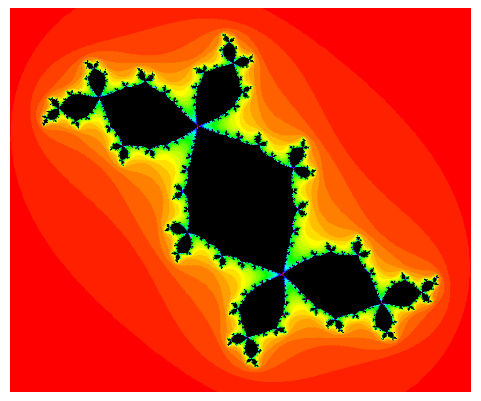
\includegraphics[scale=0.5]{./img/C3/julia-explicado-1.png} &   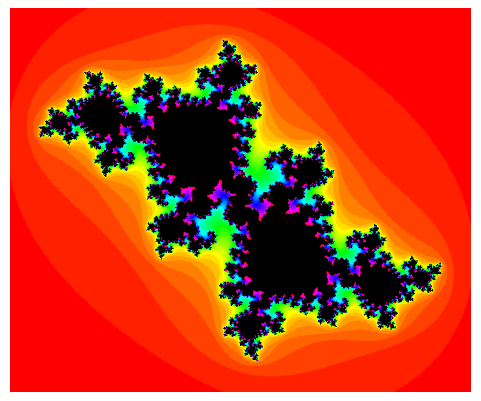
\includegraphics[scale=0.5]{./img/C3/julia-explicado-2.png} \\
  (a) $J_{-0.12+0.75i}$ & (b) $J_{-0.23+0.65i}$  \\[6pt]
  \end{tabular}
  \caption{Conjuntos de Julia graficados con Mathematica}
  \label{fig:julia-explicados}
\end{figure}

Por sí solo Mathematica incluye una función \verb|JuliaSetPlot[c]| que muestra una imagen del conjunto $\mathsf{J}_c$. Esta función permite modificar los mismos parámetros que el método que acabamos de programar por nuestra cuenta, véanse las imágenes \ref{fig:julia-set-plot}.

\begin{figure}[ht]
  \centering
  \begin{tabular}{cc}
    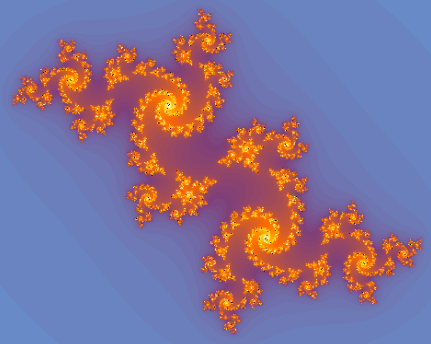
\includegraphics[scale=0.4]{./img/C3/juliaSetPlot-1.png} &   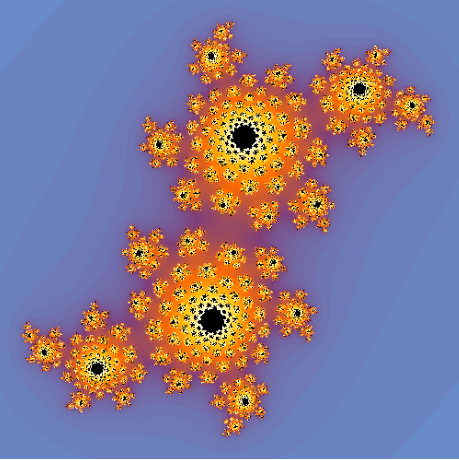
\includegraphics[scale=0.3]{./img/C3/juliaSetPlot-2.png} \\
  (a) $J_{-0.23+0.69i}$ & (b) $J_{0.16-0.59i}$  \\[6pt]
  \end{tabular}
  \caption{Resultados de la orden `JuliaSetPlot'}
  \label{fig:julia-set-plot}
\end{figure}

